\documentclass[titlepage, a4paper, 11pt, reqno, openany]{report}
%
%\begin{comment}
%a4paper leqno reqno letterpaper  a5paper b5paper executivepaper legalpaper draft amsart
%\end{comment}
%ladscape twocolumn oneside twoside
%titlepage openany
%article report book slides proc minimal amsart sample
%
\usepackage{amsfonts}
%\usepackage[brazil]{babel} %linguagem do documento
%\usepackage{babel}
\usepackage[portuguese]{babel}
\usepackage{babelbib}
%\usepackage[utf8]{inputenc} %reconhece acento e cedilha
\usepackage{amssymb}
\usepackage{latexsym}
\usepackage{amsmath}
%\usepackage[fleqn]{amsmath}
%\usepackage{mathtools}
%\usepackage[fleqn]{mathtools}
\usepackage{pxfonts} %permite simbolos matemáticos
\usepackage{mathrsfs} %permite uso de fontes para conjuntos
\usepackage[normalem]{ulem} %permite sublinhar palavras
\usepackage{mathrsfs} %permite o uso de letras trabalhadas
%\usepackage[margin=1in, paperwidth=8.5in, paperheight=11in]{geometry}
%\usepackage[top=1in, bottom=1in, left=1in, right=1in]{geometry}
%\usepackage{fullpage}
\usepackage[top=1.5cm,left=1.5cm,right=1.5cm,bottom=1.5cm]{geometry} %margens
\usepackage{graphicx} %permite inserir figuras
\usepackage[usenames]{color} %permite letras coloridas
\usepackage{makeidx} %pra criar índice remissivo
%\usepackage{tikz}
%\usepackage{pgfplots}
\usepackage{mathptmx}
%\usepackage{named}
\usepackage{enumerate}
%\usepackage{amscls}
%alguns pacotes nao sao reconhecidos, ter atencao quais usar em differents computadores.
\usepackage{float}
\usepackage{caption}
\usepackage{verbatim}
%%%%%%%%%%%%%%%%%%%%
\newtheorem{theorem}{Theorem}
\newtheorem{lemma}{Lemma}
\newtheorem{definition}{Defini\c{c}\~{a}o}
\newtheorem{notation}{Notation}
%%%%%%%%%%%%%%%%%%%%

\bibliographystyle{babplain}

\makeindex

%
\begin{document}
\begin{titlepage}
\begin{minipage}{0.95\linewidth}
\centering

\includegraphics[scale=0.60]{./image/ISEP_marca_cor_grande.png}
\label{Capa}
\title{Electr\'{o}nica de Pot\^{e}ncia}
\author{\emph{S\'{e}rgio Santos},\;$N^o$:\; 1020881}
\date{\today}
\maketitle
\end{minipage}
\end{titlepage}
%titlepage
%
\tableofcontents
%
\appendix
%
\pagestyle{plain}%plain headings empty
%
%few lessons \newline \newpage only in text.
%\pagestyle{headings} %estilo de numeração
%{\tiny text}{\scriptsize text}{\footnotesize text}{\small text}{\normalize text}{\large text}{\Large text}{\huge text}{Huge text}{\it text}{\bf text}{\tt text}\underline{text}
%\newline \newpage \linebreak \\[distance]
%\. \, \; quad qquad hspace{xx cm} vspace{xx cm}
%{\color{cor}text}
%\footcite{•}\twocolumn\onecolumn
% $ formula $ $$ formula $$ \nonumber \\
%\frac{•}{•} \dfrac{•}{•} \sqrt[•]{•} \binom{}{}
%\mathbb{NZqRC} \mathcal{texto} \mathfrak{texto}
%\vert \Vert \leq \geq \neq \to \lim
%displaystyle \int \sum \prod \cup \cap
%\longleftarrow \overline{•} \langle
%\hline \caption \label \centering \ref{Capa}
%
%%%%%%%%%%%%%%%%%%%%%%%%%%%%%%%%%%%%%%%%%%%%
\part{Problema 1 - A 1}\label{parte1}
%
\section{An\'{a}lise circuito \index{circuito} $LC$, $D-LC$ e $RLC$ em $C.C$.}
%
An\'{a}lise de transit\'{o}rios \index{transit\'{o}rios} num circuito \index{circuito} $RLC$ s\'{e}rie, alimentado por uma fonte \index{fonte} $DC$.\par
%
Considere o circuito \index{circuito}:\par
%
\begin{minipage}{0.95\linewidth}
\centering
\makebox[0.9\linewidth]{
\includegraphics[scale=0.8]%width height angle scale
{./image/Screenshot11.png}
}
\captionof{figure}{Circuito LC C.C}
\label{figura 1}
\end{minipage}\par
%
\begin{enumerate}
%1
\item
O interruptor \index{interruptor} \'{e} fechado em $t=0s$ e nesse instante $V_c=0$ (condensador \index{condensador} descarregado).\par
%
\begin{enumerate}
%1a
\item
Com os pontos \index{pontos} $A$ e $B$ em curto-circuito \index{curto-circuito}. Deduze \index{Deduze} as formas \index{formas} de onda \index{onda} da corrente \index{corrente} $i(t)$; da tens\~{a}o \index{tens\~{a}o} no condensador \index{condensador} $V_c(t)$; da tens\~{a}o \index{tens\~{a}o} na bobine \index{bobine} $V_L(t)$. Representando \index{Representando} as formas \index{formas} de onda \index{onda} obtidas \index{obtidas};\par
%
Fonte \index{Fonte} de alimenta\c{c}\~ao \index{alimenta\c{c}\~ao}\par
\begin{equation}
V_{DC}(t)=100\times u(t)
\end{equation}\par
%
Condi\c{c}\~{o}es \index{Condi\c{c}\~{o}es} iniciais \index{iniciais}\par
\[ V_c(0^-)=0 \]\par
Equa\c{c}\~{a}o \index{Equa\c{c}\~{a}o} do circuito \index{circuito}\par
%
\begin{equation}
\boxed{
V_{DC}(t)=\frac{Q_c(t)}{C}+L \cdot \frac{d i(t)}{dt}\ \ ;\ t>0^-}
\end{equation}\par
%
\begin{flalign}
Q_c(t)=&\int^ti(t) \quad dt &\\ =&Q_c(0^-)+\int_{0^-}^ti(t) \quad dt \nonumber &\\
V_{DC}(t)=&\frac{1}{C}\times\left[Q_c(0^-)+\int_{0^-}^t i(t) \quad dt\right]+L\times\frac{di(t)}{dt} &\\
=&\frac{Q_c(0^-)}{C}+\frac{\int_{0^-}^t i(t) \quad dt}{C}+L\times\frac{di(t)}{dt} \nonumber &\\
=&V_c(0^-)+\frac{\int_{0^-}^t i(t) \quad dt}{C}+L\times\frac{di(t)}{dt} \nonumber &
\end{flalign}\par
%
Aplicando agora a transformada \index{transformada} ($\mathcal{L}$) de Laplace \index{Laplace} a equa\c{c}\~{a}o \index{equa\c{c}\~{a}o} com $V_c(0^-)=0$ e $i_L(0^-)=0$\par
%
\begin{flalign}
V_{DC}(s)=&\frac{I(s)}{sC}+L\times\left[sI(s)-i_L(0^-) \right] & \\
=&\frac{I(s)}{sC}+LsI(s) \nonumber & \\
\frac{100}{s}=&\left[ \frac{1}{sC}+Ls \right]\times I(s) & \\
=&\left[ \frac{LCs^2+1}{sC} \right]\times I(s) \nonumber & \\
=&\left[ \frac{s^2+\frac{1}{LC}}{\frac{s}{L}} \right]\times I(s) \nonumber & \\
=&\left[ \frac{L(s^2+\frac{1}{LC})}{s} \right]\times I(s) \nonumber & \\
100=&\left[ L(s^2+\frac{1}{LC}) \right]\times I(s) & \\
I(s)=&\frac{\frac{100}{L}}{s^2+\frac{1}{LC}} & \\
=&\left.K_1\times\frac{\frac{1}{\sqrt{LC}}}{s^2+\left( \frac{1}{\sqrt{LC}} \right)^2}\right|_{K_1=\frac{100\sqrt{LC}}{L}} \ \ \ Roc>0 \nonumber &
\end{flalign}\par
%
Da como resultado \index{resultado} sua corrente \index{corrente},\par
%
\begin{equation}
i(t)=10\sin{\frac{t}{\sqrt{LC}}}\ u(t)
\end{equation}\par
%
A tens\~{a}o \index{tens\~{a}o} na bobine \index{bobine} $V_L(t)=L\frac{d i(t)}{dt}$, isto \'{e},\par
%
\begin{equation}
V_L(t)=100\cos{\frac{t}{\sqrt{LC}}}\ u(t)
\end{equation}\par
%
A tens\~{a}o \index{tens\~{a}o} no condensador \index{condensador} $V_c(t)=\frac{1}{C}\int_{0^-}^ti(t)$, isto \'{e},\par
%
\begin{equation}
V_c(t)=100 \left(1-\cos{\frac{t}{\sqrt{LC}}}\right)\ u(t)
\end{equation}\par
%
Representa\c{c}\~{a}o \index{Representa\c{c}\~{a}o} gr\'{a}fica \index{gr\'{a}fica}:\par
%
\begin{figure}[H]
%h t b H !h
\centering
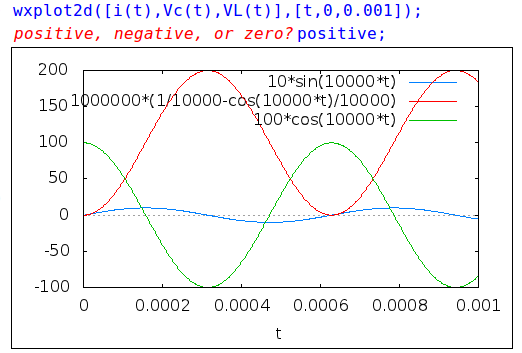
\includegraphics[scale=0.80]{./image/electpt2.png}
\caption{{\color{red}$V_c(t)$}\quad e \quad {\color{green}$V_L(t)$} \quad e \quad{\color{blue}$i(t)$}}
\label{figura 2}
\end{figure}
%1b
\item
Supondo \index{Supondo} agora que entre $A$ e $B$ \'{e} colocado \index{colocado} um d\'{i}odo \index{d\'{i}odo} com o C\'{a}todo \index{C\'{a}todo} ligado \index{ligado} a $A$.\par
%
Como o d\'{i}odo \index{d\'{i}odo} s\'{o} conduz \index{conduz} numa direc\c{c}\~{a}o \index{direc\c{c}\~{a}o}, n\~{a}o existe for\c{c}a \index{for\c{c}a} contra eletromotriz \index{eletromotriz} da bobine \index{bobine}, ou seja, a corrente \index{corrente} s\'{o} flui numa direc\c{c}\~{a}o \index{direc\c{c}\~{a}o}, isto \'{e}, s\'{o} existe meio ciclo \index{ciclo} da onda \index{onda} sinusoidal \index{sinusoidal} j\'{a} obtida no exerc\'{i}cio anterior.\par
%
\[
i(t)=
\begin{cases}
10\sin{\frac{1}{\sqrt{LC}}t},
&\text{if \quad $0 \leq t < \frac{T_0}{2}$;}\\
0,
&\text{if \quad $t \geq \frac{T_0}{2}$;}\\
\end{cases}
\]\par
%
A partir de \quad $t \geq \frac{T_0}{2}$ \quad condi\c{c}\~{o}es inicias \quad $V_c(\frac{T_0}{2}^-)=200$ \quad e \quad $V_L(\frac{T_0}{2}^-)=-100$\par
%condensador
\begin{flalign}
V_c(t) =& V_c(\frac{T_0}{2}^-)+\frac{\int_{\frac{T_0}{2}^-}^t i(t)}{C} & \\
=& V_c(\frac{T_0}{2}^-)+0 \nonumber & \\
=& 200 \times u \left(t-\frac{T_0}{2} \right) \nonumber & \\
%bobine
V_L(t) =& L \dfrac{d i(t)}{dt} & \\
=& 0 \times u \left(t-\frac{T_0}{2} \right) \nonumber &
\end{flalign}\par
%graphico
Representa\c{c}\~{a}o gr\'{a}fica:\par
\begin{figure}[H]
\centering
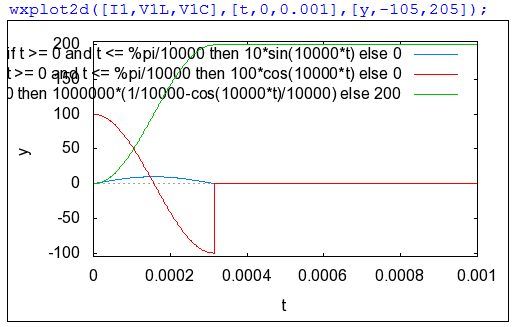
\includegraphics[scale=0.95]{./image/electpt5.png}
\caption{Circuito LC com d\'{i}odo em C.C}
\label{figura 3}
\end{figure}
%
Na qual ao chegar e ap\'{o}s a $t=\frac{\pi}{10000}$ a tens\~{a}o \index{tens\~{a}o} do \textcolor{red}{condensador} \index{condensador} continua \index{continua} nos $200V$ e a tens\~{a}o \index{tens\~{a}o} na \textcolor{green}{bobine} \index{bobine} e a \textcolor{blue}{corrente} \index{corrente} s\~{a}o nulos \index{nulos}.\par
%1c
\item
Supondo \index{Supondo} que o d\'{i}odo \index{d\'{i}odo} \'{e} substitu\'{i}do por uma resist\^{e}ncia \index{resist\^{e}ncia} $R$, determine o valor da resist\^{e}ncia \index{resist\^{e}ncia} de modo a que o circuito \index{circuito} tenha um comportamento \index{comportamento} n\~{a}o oscilat\'{o}rio \index{oscilat\'{o}rio}.\par
%
Equa\c{c}\~{a}o \index{Equa\c{c}\~{a}o} do circuito \index{circuito}\par
%
\begin{equation}
\boxed{
V_{DC}(t)=\frac{Q_c(t)}{C}+L\frac{d i(t)}{dt}+R\ i(t)\ \ ;\ t>0^-}
\end{equation}\par
%\fbox{text}
%
Aplicando \index{Aplicando} a Transformada \index{Transformada} de Laplace \index{Laplace}, supondo que as condi\c{c}\~{o}es iniciais \index{iniciais} s\~{a}o nulas \index{nulas}\par
%
\begin{flalign}
\frac{V_{DC}(s)}{I(s)}=&Ls+\frac{1}{sC}+R\ \ ;\ Roc>0^- & \\
\frac{V_{DC}(s)Cs}{I(s)}=&LCs^2+RCs+1 & \\
\frac{V_{DC}(s)s}{I(s)L}=&s^2+\frac{R}{L}s+\frac{1}{LC} & \\
I(s)=&\frac{100/L}{s^2+\frac{R}{L}s+\frac{1}{LC}} &
\end{flalign}\par
%
Desta Equa\c{c}\~{a}o \index{Equa\c{c}\~{a}o} sabemos que:\par
%
$2 \xi \omega_n = \frac{R}{L}$\; ; \qquad
$\omega_n^2=\frac{1}{LC}$\; ; \qquad
$\omega_d=w_n\sqrt{1-\xi^2}$\par
e que:\par
%
$Subamortecido\implies 0\leq \xi <1$\par
$Amortecido\ critico\implies \xi =1$\par
$Sobreamortecido\implies \xi >1$\par
$$\therefore$$
$$para\  \xi = 1$$
%
\begin{equation}
2\omega_n=\frac{R}{L}\ \ ou\ \ \left(\frac{R}{L}\right)^ 2-4\times \frac{1}{LC}=0\\
\end{equation}\par
%
logo o valor resistivo \index{resistivo} \'{e} 20 $\Omega$ (ohm)\par
%
\begin{flalign}
I(s)=&\frac{\frac{100}{L}}{(s+\frac{R}{2L})^2}\quad, Roc>\frac{-R}{2L} & \\
i(t)=&\frac{100}{L}\quad e^{-\frac{R}{2L}t}\ t\times u(t) &\\
=&100000\,\,t\quad e^{-10000 t}\times u(t) \nonumber &
\end{flalign}\par
%
Representa\c{c}\~{a}o \index{Representa\c{c}\~{a}o} gr\'{a}fica \index{gr\'{a}fica}:\par
%
\begin{figure}[H]
\centering
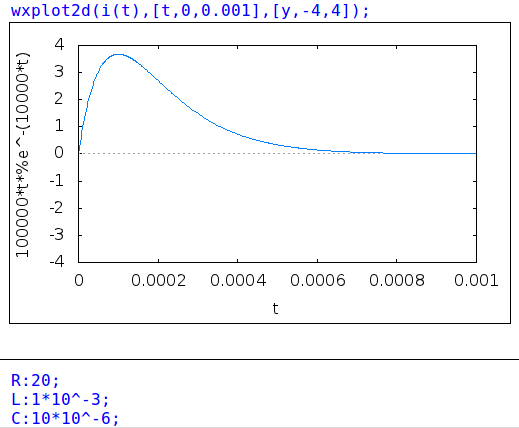
\includegraphics[scale=0.8]{./image/electpt4.png}\\
\caption{Circuito RLC Amortecido cr\'{i}tico C.C}
\label{figura 4}
\end{figure}
%
\end{enumerate}
\end{enumerate}
%
\begin{abstract}
Foram Efetuado \index{Efetuado} todas as dedu\c{c}\~{o}es \index{dedu\c{c}\~{o}es} matem\'{a}ticas \index{matem\'{a}ticas} necess\'{a}rias de modo a explicar \index{explicar} convenientemente a evolu\c{c}\~{a}o \index{evolu\c{c}\~{a}o} da corrente \index{corrente} $i(t)$ e tens\~{o}es \index{tens\~{o}es} $V_c(t)$ e $V_L(t)$, e obtido as formas \index{formas} de onda \index{onda} com base nas express\~{o}es \index{express\~{o}es} matem\'{a}ticas \index{matem\'{a}ticas}, como demonstrado \index{demonstrado} na Parte \, \index{Parte} \ref{eq}.
\end{abstract}
%
\appendix
\part{Problema 1 - A 2}
\section{Simula\c{c}\~{a}o \index{Simula\c{c}\~{a}o} no {\bf PSIM}.}
\begin{enumerate}
%1
\item
Simula\c{c}\~{a}o \index{Simula\c{c}\~{a}o} no {\bf PSIM} os circuitos/problema \index{circuitos} apresentado \index{apresentado} na Parte \ref{parte1}. Registando \index{Registando} a formas \index{formas} de onda \index{onda} e comparando \index{comparando} os resultados \index{resultados}.\par
%
\begin{figure}[H]
\centering
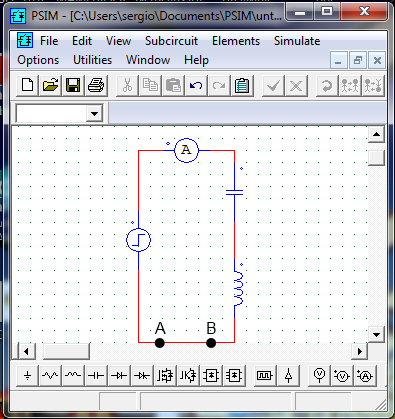
\includegraphics[scale=1.3]{./image/PSIM_0.png}
\caption{Programa $PSIM$}
\label{figura 5}
\end{figure}\par
%
\begin{enumerate}
%1a
\item
Ensaio \index{Ensaio} com curto-circuito \index{curto-circuito} entre $A$ e $B$\par
%
\begin{figure}[H]
\centering
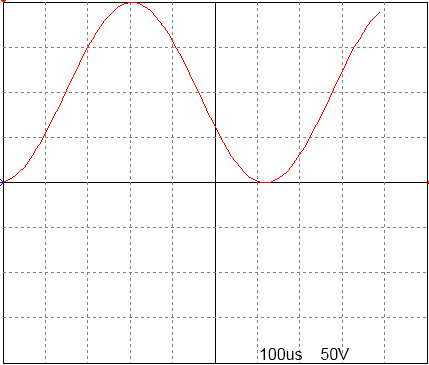
\includegraphics[scale=1]{./image/PSIM_1.png}
\caption{$V_c(t)$}
\label{figura 6}
\end{figure}\par
%
\begin{figure}[H]
\centering
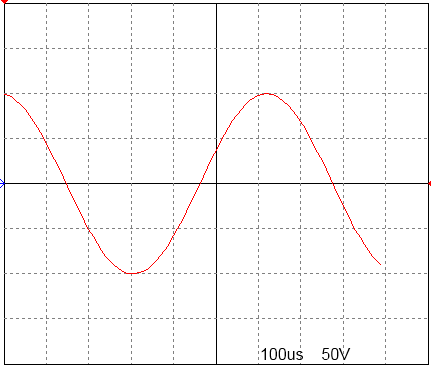
\includegraphics[scale=1]{./image/PSIM_2.png}
\caption{$V_L(t)$}
\label{figura 7}
\end{figure}\par
%
\begin{figure}[H]
\centering
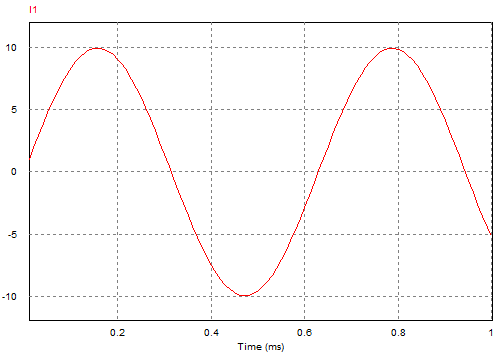
\includegraphics[scale=1]{./image/PSIM_3.png}
\caption{$i(t)$}
\label{figura 8}
\end{figure}\par
%1b
\item
Ensaio \index{Ensaio} com d\'{i}odo \index{d\'{i}odo} entre $A$ e $B$\\
Aqui existe uma differen\c{c}a \index{differen\c{c}a} com o modelo \index{modelo} matem\'{a}tico \index{matem\'{a}tico}, pois $V_L(t)$ tem um declive \index{declive} para {\color{blue} zero} depois de $t\geq\frac{T_0}{2}$.\par
%
\begin{figure}[H]
\centering
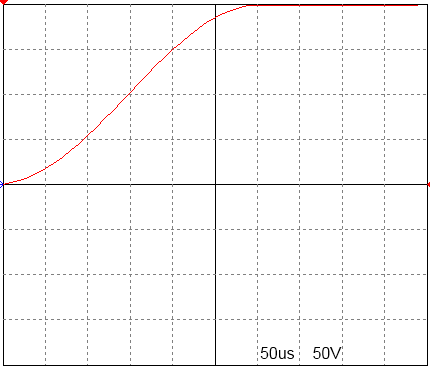
\includegraphics[scale=1]{./image/PSIM_4.png}
\caption{$V_c(t)$}
\label{figura 9}
\end{figure}\par
%
\begin{figure}[H]
\centering
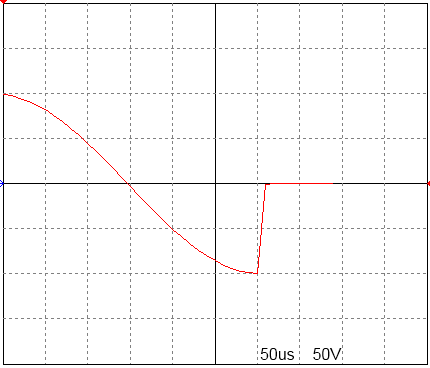
\includegraphics[scale=1]{./image/PSIM_5.png}
\caption{$V_L(t)$}
\label{figura 10}
\end{figure}\par
%
\begin{figure}[H]
\centering
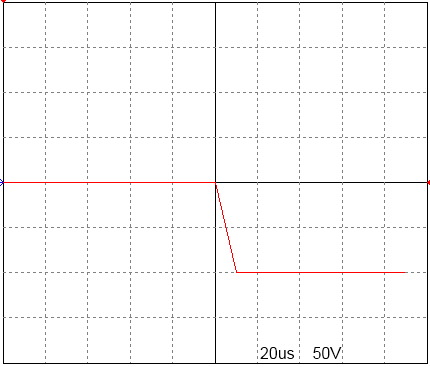
\includegraphics[scale=1]{./image/PSIM_6.png}
\caption{$V_D(t)$}
\label{figura 11}
\end{figure}\par
%
\begin{figure}[H]
\centering
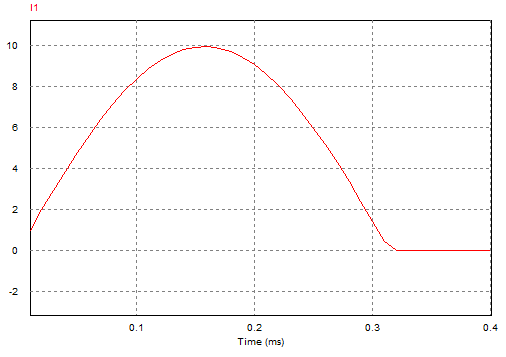
\includegraphics[scale=1]{./image/PSIM_7.png}
\caption{$i(t)$}
\label{figura 12}
\end{figure}\par
%1c
\item
Ensaio \index{Ensaio} com Resist\^{e}ncia \index{Resist\^{e}ncia} de 20 $\Omega$ (ohm) entre $A$ e $B$\par
%
\begin{figure}[H]
\centering
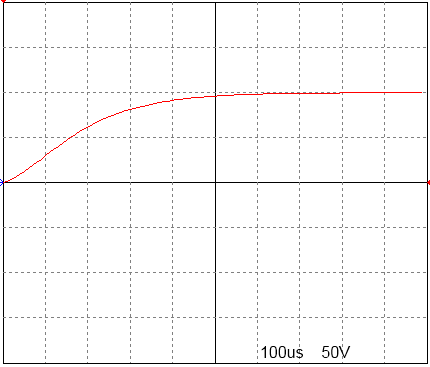
\includegraphics[scale=1]{./image/PSIM_8.png}
\caption{$V_c(t)$}
\label{figura 13}
\end{figure}\par
%
\begin{figure}[H]
\centering
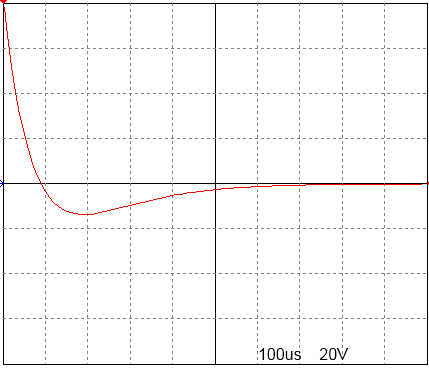
\includegraphics[scale=1]{./image/PSIM_9.png}
\caption{$V_L(t)$}
\label{figura 14}
\end{figure}\par
%
\begin{figure}[H]
\centering
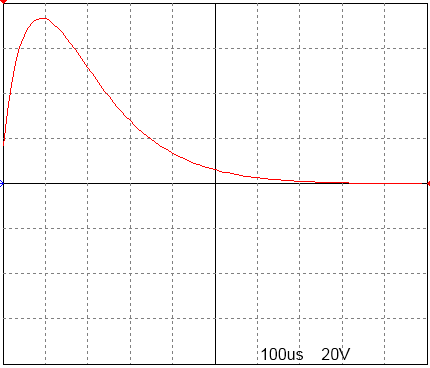
\includegraphics[scale=1]{./image/PSIM_10.png}
\caption{$V_R(t)$}
\label{figura 15}
\end{figure}\par
%
\begin{figure}[H]
\centering
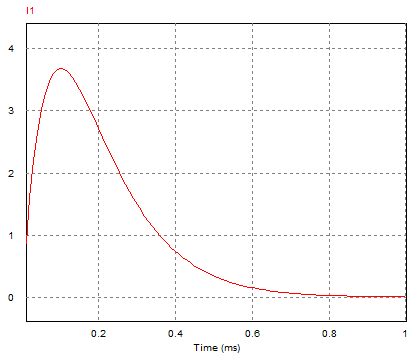
\includegraphics[scale=1]{./image/PSIM_11.png}
\caption{$i(t)$}
\label{figura 16}
\end{figure}\par
%
\end{enumerate}
%2
\item
Considerado \index{Considerado} o circuito \index{circuito}. O interruptor \index{interruptor} \'{e} fechado \index{fechado} em $t=0 s$.\par
%
\begin{minipage}{0.95\linewidth}
%\centering
\makebox[0.9\linewidth]{
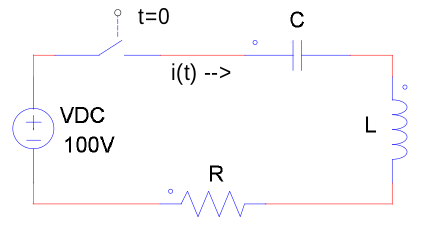
\includegraphics[scale=0.8]{./image/Screenshot12.png}
}
\captionof{figure}{Circuito RLC em C.C}
\label{figura 17}
\end{minipage}\par
%
Socorrendo \index{Socorrendo} ao Excel (ou equivalente OpenOffice), s\~{a}o representadas \index{representadas} as formas \index{formas} de onda \index{onda} da corrente \index{corrente} i(t) para os seguintes valores \index{valores} de R, L e C:\par
%
\begin{enumerate}
%2a
\item
R=2$\Omega$\ \  L=1H\ \  C=0,01F\par
\begin{figure}[H]
\centering
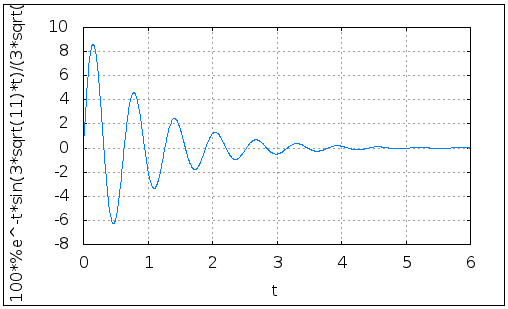
\includegraphics[scale=0.8]{./image/image_a.png}
\caption{$\xi=0.1$}
\label{figura 18}
\end{figure}\par
%2b
\item
R=2$\Omega$\ \  L=1H\ \  C=0,1F\par
\begin{figure}[H]
\centering
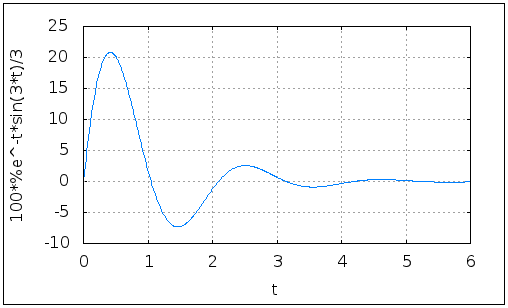
\includegraphics[scale=0.8]{./image/image_b.png}
\caption{$\xi=0.31622776601684$}
\label{figura 19}
\end{figure}\par
%2c
\item
R=2$\Omega$\ \  L=1H\ \  C=0,5F\par
\begin{figure}[H]
\centering
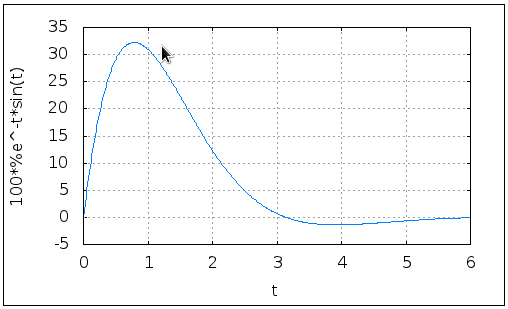
\includegraphics[scale=0.8]{./image/image_c.png}
\caption{$\xi=0.707106781188655$}
\label{figura 20}
\end{figure}\par
%2d
\item
R=2$\Omega$\ \  L=1H\ \  C=1F\par
\begin{figure}[H]
\centering
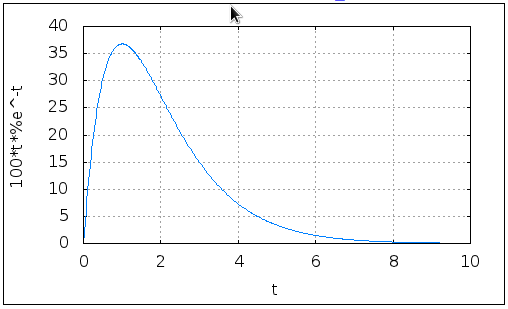
\includegraphics[scale=0.8]{./image/image_d.png}
\caption{$\xi=1$}
\label{figura 21}
\end{figure}\par
%2e
\item
R=2$\Omega$\ \  L=1H\ \  C=3F\par
\begin{figure}[H]
\centering
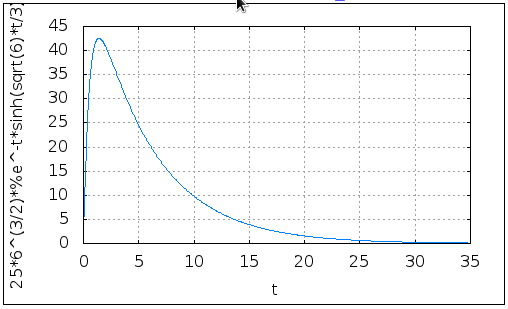
\includegraphics[scale=0.8]{./image/image_e.png}
\caption{$\xi=\sqrt{3}$}
\label{figura 22}
\end{figure}\par
%2f
\item
R=0$\Omega$\ \  L=1H\ \  C=0,5F\par
\begin{figure}[H]
\centering
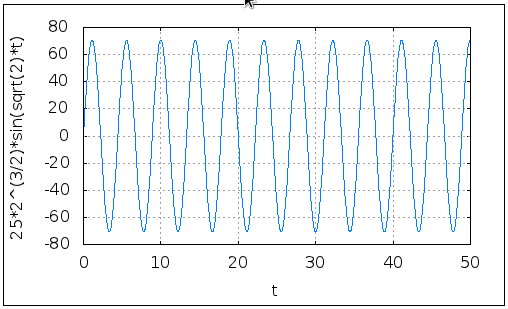
\includegraphics[scale=0.8]{./image/image_f.png}
\caption{$\xi=0$}
\label{figura 23}
\end{figure}\par
%
{Formas \index{Formas} de onda \index{onda} obtidas classificadas \index{classificadas} no que diz respeito \index{respeito} ao seu amortecimento \index{amortecimento}}\par
%
\begin{equation}
\xi=\frac{R\sqrt{LC}}{2L}
\end{equation}
%
\end{enumerate}
%3
\item
Simula\c{c}\~{a}o \index{Simula\c{c}\~{a}o} no {\bf PSIM} o problema \index{problema} apresentado \index{apresentado} no ponto anterior. Registando \index{Registando} a formas \index{formas} de onda \index{onda} e comparando \index{comparando} os resultados \index{resultados}.\par
%
\begin{enumerate}
%3a
\item
R=2$\Omega$\ \  L=1H\ \  C=0,01F\par
\begin{figure}[H]
\centering
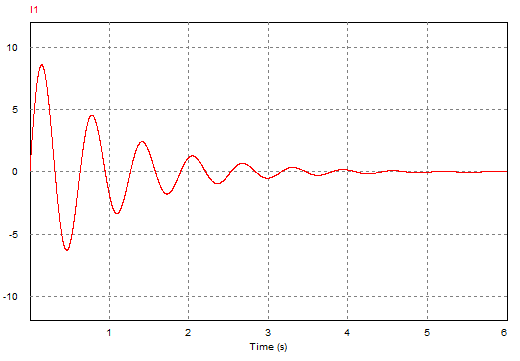
\includegraphics[scale=1]{./image/PSIM_12.png}
\caption{$\xi=0.1$}
\label{figura 24}
\end{figure}\par
%3b
\item
R=2$\Omega$\ \  L=1H\ \  C=0,1F\par
\begin{figure}[H]
\centering
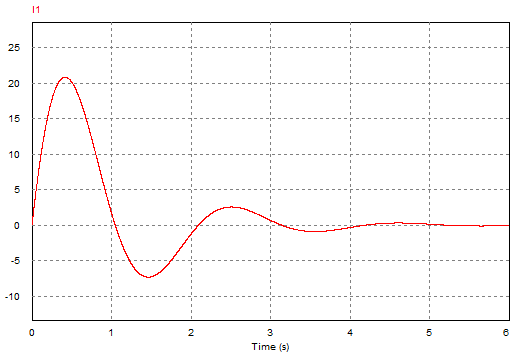
\includegraphics[scale=1]{./image/PSIM_13.png}
\caption{$\xi=0.31622776601684$}
\label{figura 25}
\end{figure}\par
%3c
\item
R=2$\Omega$\ \  L=1H\ \  C=0,5F\par
\begin{figure}[H]
\centering
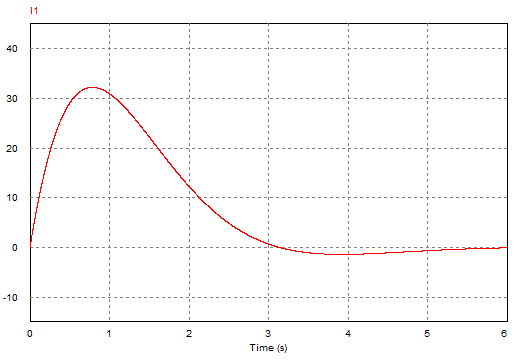
\includegraphics[scale=1]{./image/PSIM_14.png}
\caption{$\xi=0.707106781188655$}
\label{figura 26}
\end{figure}\par
%3d
\item
R=2$\Omega$\ \  L=1H\ \  C=1F\par
\begin{figure}[H]
\centering
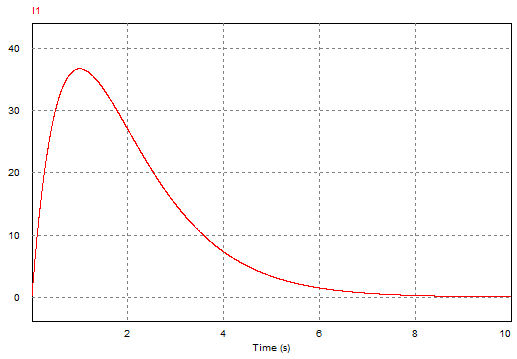
\includegraphics[scale=1]{./image/PSIM_15.png}
\caption{$\xi=1$}
\label{figura 27}
\end{figure}\par
%3e
\item
R=2$\Omega$\ \  L=1H\ \  C=3F\par
\begin{figure}[H]
\centering
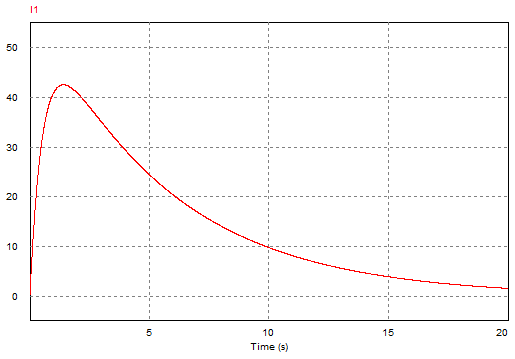
\includegraphics[scale=1]{./image/PSIM_16.png}
\caption{$\xi=\sqrt{3}$}
\label{figura 28}
\end{figure}\par
%3f
\item
R=0$\Omega$\ \  L=1H\ \  C=0,5F\par
\begin{figure}[H]
\centering
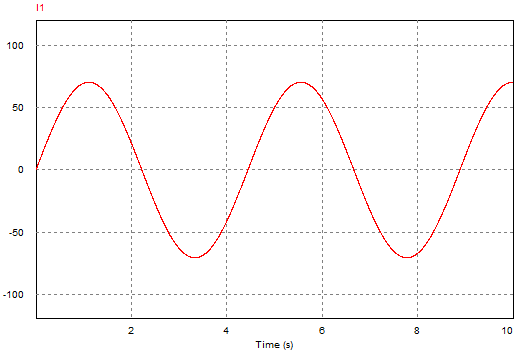
\includegraphics[scale=1]{./image/PSIM_17.png}
\caption{$\xi=0$}
\label{figura 29}
\end{figure}\par
%
\end{enumerate}
\end{enumerate}
%
\begin{abstract}
Foi apresentado \index{apresentado} os c\'{a}lculos \index{c\'{a}lculos}  \index{matem\'{a}ticos}, formas de onda \index{onda} pelo modelo \index{modelo} matem\'{a}tico \index{matem\'{a}tico} e pelo simulador \index{simulador} {\bf PSIM}, na situa\c{c}\~{a}o \index{situa\c{c}\~{a}o} da Figura \ref{figura 1} em curto-circuito \index{curto-circuito}, com resist\^{e}ncia \index{resist\^{e}ncia} em amortecimento \index{amortecimento} cr\'{i}tico \index{cr\'{i}tico} e com d\'{i}odo \index{d\'{i}odo}, mostrando os comportamentos \index{comportamentos} das vari\'{a}veis \index{vari\'{a}veis} Tens\~{a}o \index{Tens\~{a}o} e Corrente \index{Corrente}, depois foi feito o estudo da Figura \ref{figura 17} circuito \index{circuito} $RLC$ nos seus estados \index{estados} de amortecimento \index{amortecimento} ($\xi$) e respetivo comportamento \index{comportamento} das suas vari\'{a}veis \index{vari\'{a}veis}, os valores \index{valores} obtidos sendo iguais \index{iguais} pela representa\c{c}\~{a}o \index{representa\c{c}\~{a}o} matem\'{a}tica \index{matem\'{a}tica} e simulador \index{simulador} {\bf PSIM}.
\end{abstract}
\newpage
\part{Equa\c{c}\~{o}es} \label{eq}
%
\begin{flushleft}
{\bf Corrente Continua Condi\c{c}\~{o}es \index{Condi\c{c}\~{o}es} iniciais \index{iniciais} nulas \index{nulas}.}\par
\end{flushleft}
 \quad Circuito \index{Circuito} $LC$ em $C.C$:\par
%
\begin{itemize}
\item
$i(t)=\frac{V_{DC}\sqrt{LC}}{L}\quad \sin \left( \frac{t}{\sqrt{LC}}\right)\times u(t)$\par
\item
$V_L(t)=V_{DC}\quad \cos\left(\frac{t}{\sqrt{LC}} \right)\times u(t)$\par
\item
$V_c(t)=V_{DC}\quad \left(1-\cos\left(\frac{t}{\sqrt{LC}} \right) \right)\times u(t)$\par
\item
$\omega_n=\frac{1}{\sqrt{LC}}$\par
\item
$\overline{Z}=\sqrt{(\omega_n L-\frac{1}{\omega_n C})^2}$\par
\item
$\phi_p=\frac{\pi}{2}$\par
porque, $\sin(\omega_n t)= \cos(\omega_n t - \pi/2)$\par
\item
$\tau=\infty$\par
\end{itemize}
%
%%%%%%%%%%%%%%%%%%%%%
\quad Circuito \index{Circuito} $RLC$ em $C.C$:\par
%
\begin{enumerate}
%enum1
\item
Para \quad $C(C R^2-4 L)>0$ \quad (Ra\'{i}zes \index{Ra\'{i}zes} reais \index{reais} diferentes \index{diferentes}) \quad Sobreamortecido \index{Sobreamortecido}.\par
%
\begin{itemize}
\item
$i(t)=\frac{2 V_{DC} C e^{\frac{-tR}{2L}} sinh \left( \frac{t \sqrt{C(CR^2-4L)}}{2CL} \right)}{\sqrt{C(CR^2-RL)}}\times u(t)$\par
\item
$V_R(t)=R\times i(t)$\par
\item
$V_L(t)=L\dfrac{di(t)}{dt}$\par
%
\begin{minipage}{0.95\linewidth}
\makebox[\linewidth]{
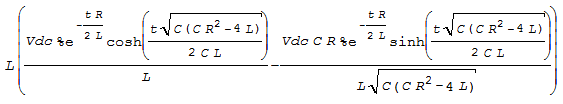
\includegraphics[scale=0.75]{./image/equacoes_1.png}
}
\end{minipage}\par
%
\item
$V_C(t)=\frac{1}{C}\int_0^ti(t)$\par
%
\begin{minipage}{0.95\linewidth}
\makebox[\linewidth]{
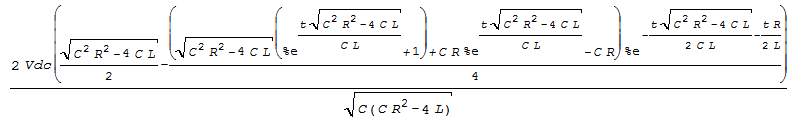
\includegraphics[scale=0.75]{./image/equacoes_2.png}
}
\end{minipage}\par
%
\end{itemize}
%enum2
\item
Para \quad $C(C R^2-4 L)=0$ \quad (Ra\'{i}zes \index{Ra\'{i}zes} iguais \index{iguais})\quad Amortecimento \index{Amortecimento} cr\'{i}tico \index{cr\'{i}tico}.\par
%
\begin{itemize}
\item
$i(t)=\frac{V_{DC}}{L} \quad  t \quad e^{\frac{-R t}{2L}} \times u(t)$\par
\item
$V_R(t)=R\times i(t)$\par
\item
$V_L(t)=L\dfrac{di(t)}{dt}$\par
%
\begin{minipage}{0.95\linewidth}
\makebox[\linewidth]{
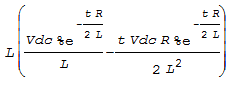
\includegraphics[scale=0.75]{./image/equacoes_3.png}
}
\end{minipage}\par
%
\item
$V_C(t)=\frac{1}{C}\int_0^ti(t)$\par
\begin{minipage}{0.95\linewidth}
\makebox[\linewidth]{
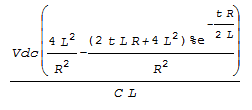
\includegraphics[scale=0.75]{./image/equacoes_4.png}
}
\end{minipage}\par
%
\end{itemize}
%enum3
\item
Para \quad $C(C R^2-4 L)<0$ \quad (Ra\'{i}zes \index{Ra\'{i}zes} complexas \index{complexas}) \quad Amortecido \index{Amortecido}.\par
%
\begin{itemize}
\item
$i(t)=\frac{2 V_{DC} C e^{\frac{-tR}{2L}} sin \left( \frac{t \sqrt{-C(CR^2-4L)}}{2CL} \right)}{\sqrt{-C(CR^2-4L)}}\times u(t)$\par
\item
$V_R(t)=R\times i(t)$\par
\item
$V_L(t)=L\dfrac{di(t)}{dt}$\par
%
\begin{minipage}{0.95\linewidth}
\makebox[\linewidth]{
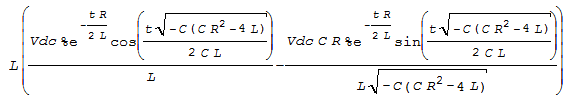
\includegraphics[scale=0.75]{./image/equacoes_5.png}
}
\end{minipage}\par
%
\item
$V_C(t)=\frac{1}{C}\int_0^ti(t)$\par
%
\begin{minipage}{0.95\linewidth}
\makebox[\linewidth]{
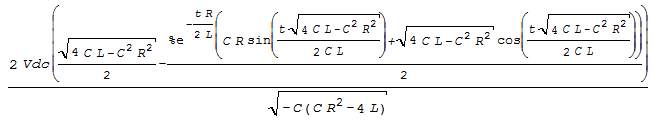
\includegraphics[scale=0.75]{./image/equacoes_6.png}
}
\end{minipage}\par
%
\end{itemize}
\end{enumerate}
%
\begin{itemize}
\item
$| \omega_n |=\sqrt{\frac{4 L-R^2 C}{4 L^2 C}}$\par
\item
%\overrightarrow{Z}
$\overline{Z}=\sqrt{R^2 + (\omega_n L -\frac{1}{\omega_n C})^2}$\par
\item
$\phi_p=\arctan\left(\frac{\omega_n L - \frac{1}{\omega_n C}}{R}\right)$\par
\item
$\tau=\frac{2 L}{R}$\par
\end{itemize}
%%%%%%%%%%%%%%%%%%%%%%%%%%%%%%%%%%%%%%%%%%
\begin{flushleft}
{\bf Corrente \index{Corrente} Alternada condi\c{c}\~{o}es \index{Condi\c{c}\~{o}es} iniciais \index{iniciais} nulas \index{nulas}}.
\end{flushleft}
\quad Circuito \index{Circuito} $RLE$ em $C.A$:\par
\begin{itemize}
\item
$i(t)=C_T\ e^{-\frac{R}{L}t}+\frac{V_{m\acute{a}x}}{\overline{Z}}\sin(\omega t + \alpha - \phi_p)-\frac{E}{R}$\newline
$i(t)=C_T\ e^{-\frac{R}{L}t} + C_1 \cos (\omega t) + C_2 \sin(\omega t)-\frac{E}{R}$
\item
$I(\omega t)=C_T\ e^{-\frac{R}{L \omega}\omega t}+\frac{V_{m\acute{a}x}}{\overline{Z}}\sin(\omega t + \alpha - \phi_p)-\frac{E}{R}$
\item
$\overrightarrow{Z}=R+j\omega L$\\
$\overline{Z}=\sqrt{R^2 + (\omega L)^2}$
\item
$\phi_p=\arctan(\frac{\omega L}{R})$
\item
$C_T=\frac{E}{R}-\frac{V_{m\acute{a}x}}{\overline{Z}}\sin(\alpha - \phi_p)$
\item
$C_T=\frac{V_{m\acute{a}x}}{R^2 + (\omega L)^2}(L \omega \cos(\alpha) - R \sin (\alpha))+\frac{E}{R}$
\item
$C_1=\frac{V_{m\acute{a}x}}{R^2 + (\omega L)^2}(R \sin (\alpha) - L \omega \cos(\alpha))$
\item
$C_2=\frac{V_{m\acute{a}x}}{R^2 + (\omega L)^2}(R \cos (\alpha) + L \omega \sin (\alpha))$
%
\end{itemize}
%%%%%%%%%%%%%%%%%%%%%%%%%%%%%%%%%%
\begin{definition}
Capacit\^{a}ncia
\begin{flalign*}
Q_c(t) =& \int^t i(t) \quad dt & \\
=& Q_c(0^-)+\int_{0^-}^t i(t) \quad dt & \\
V_c(t) =& \frac{Q_c(t)}{C} & \\
=& \frac{1}{C} \quad \int^t i_c(t) \quad dt & \\
=& \frac{Q_c(0^-)}{C} + \frac{1}{c} \quad \int_0^t i_c(t) \quad dt & \\
=& V(0^-) + \frac{1}{c} \quad \int_0^t i_c(t) \quad dt & \\
i_c(t) =& C \quad \dfrac{d V_c(t)}{dt} &
\end{flalign*}\par
\end{definition}
%
\begin{definition}
Indut\^{a}ncia
\begin{flalign*}
\psi_L(t) =& \int^t V_L(t) \quad dt & \\
=& \psi_L(0^-)+\int_{0^-}^t V_L(t) \quad dt & \\
V_L(t) =& L \quad \dfrac{d i_L(t)}{dt} & \\
i_L(t) =& \frac{\psi_L(t)}{L} & \\
=& \frac{1}{L} \quad \int^t V_L(t) \quad dt & \\
=& \frac{\psi_L(0^-)}{L} + \frac{1}{L} \quad \int_0^t V_L(t) \quad dt & \\
=& i_L(0^-) + \frac{1}{L} \quad \int_0^t V_L(t) \quad dt &
\end{flalign*}\par
\end{definition}
%
\begin{definition}
Resist\^{e}ncia
\begin{flalign*}
V_R(t) =& R \quad i_R(t) & \\
i_R(t) =& \frac{V_R(t)}{R} &
\end{flalign*}\par
\end{definition}
%
\begin{definition}
Valor M\'{e}dio
\begin{flalign*}
X_{av} =& \frac{1}{T} \; \int_0^T X(t) dt &
\end{flalign*}\par
\end{definition}
%
\begin{definition}
Valor Eficaz
\begin{flalign*}
X_{ef} =& \sqrt{ \frac{1}{T} \; \int_0^T \overset{\text{2}}{X(t)} dt } &
\end{flalign*}\par
\end{definition}
%

%%%%%%%%%%%%%%%%%%%%%%%%%%%%%%%%%%%%%%%%%%%
\newpage
\listoffigures
\cite{*}
\bibliography{./bibliography/Bibliography}
%\printindex
\newpage
\footnote{Apontamentos Electr\'{o}nica de Pot\^{e}ncia}
\end{document}
